\documentclass[tikz,border=10pt]{standalone}
\usepackage{tikz}
\usetikzlibrary{patterns}

\begin{document}
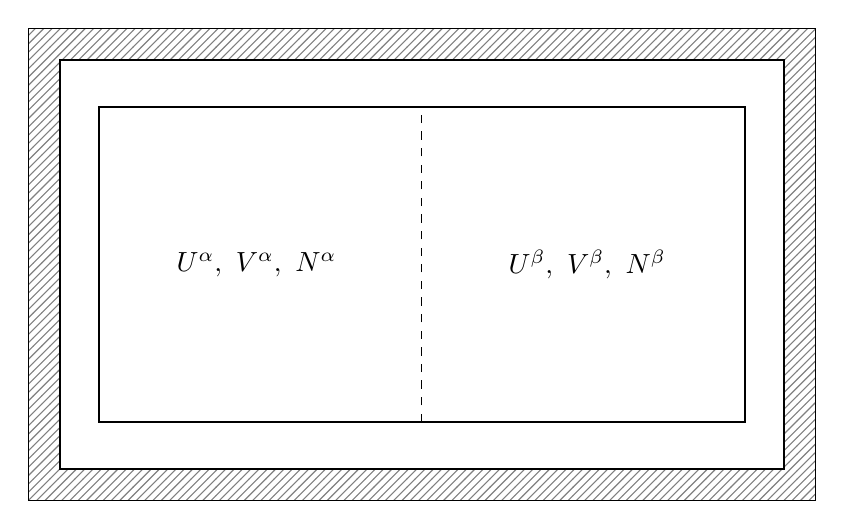
\begin{tikzpicture}
    % Outer insulated boundary
    \draw[pattern=north east lines, pattern color=black!50] (0,0) rectangle (10,6);
    \fill[white] (0.4,0.4) rectangle (9.6,5.6);
    \draw[thick] (0.4,0.4) rectangle (9.6,5.6);

    % Combined region with open boundary
    \draw[thick] (0.9,1.0) rectangle (9.1,5.0);
    \draw[dashed] (5.0,1.0) -- (5.0,5.0);

    % Labels
    \node at (2.9,3.0) {$U^\alpha,\ V^\alpha,\ N^\alpha$};
    \node at (7.1,3.0) {$U^\beta,\ V^\beta,\ N^\beta$};
\end{tikzpicture}
\end{document}
